% This must be in the first 5 lines to tell arXiv to use pdfLaTeX, which is strongly recommended.
\pdfoutput=1
% In particular, the hyperref package requires pdfLaTeX in order to break URLs across lines.

\documentclass[11pt]{article}

\usepackage[natbibapa,nodoi]{apacite}
\bibliographystyle{apacite}

\usepackage{graphicx}
\graphicspath{ {../images/} }

% Remove the "review" option to generate the final version.
\usepackage[]{ACL2023}

% Standard package includes
\usepackage{times}
\usepackage{latexsym}

% For proper rendering and hyphenation of words containing Latin characters (including in bib files)
\usepackage[T1]{fontenc}

% This assumes your files are encoded as UTF8
\usepackage[utf8]{inputenc}

% This is not strictly necessary, and may be commented out.
% However, it will improve the layout of the manuscript,
% and will typically save some space.
\usepackage{microtype}

% This is also not strictly necessary, and may be commented out.
% However, it will improve the aesthetics of text in
% the typewriter font.
\usepackage{inconsolata}


% If the title and author information does not fit in the area allocated, uncomment the following
%
%\setlength\titlebox{<dim>}
%
% and set <dim> to something 5cm or larger.

\title{Text-to-SQL Generation for Information Retrieval}

% Author information can be set in various styles:
% For several authors from the same institution:
% \author{Author 1 \and ... \and Author n \\
%         Address line \\ ... \\ Address line}
% if the names do not fit well on one line use
%         Author 1 \\ {\bf Author 2} \\ ... \\ {\bf Author n} \\
% For authors from different institutions:
% \author{Author 1 \\ Address line \\  ... \\ Address line
%         \And  ... \And
%         Author n \\ Address line \\ ... \\ Address line}
% To start a seperate ``row'' of authors use \AND, as in
% \author{Author 1 \\ Address line \\  ... \\ Address line
%         \AND
%         Author 2 \\ Address line \\ ... \\ Address line \And
%         Author 3 \\ Address line \\ ... \\ Address line}

\author{
    Jacob Waffle \\
    Boise State University\\
    \texttt{jakewaffle@u.boisestate.edu} \\
}

\begin{document}
\maketitle
\begin{abstract}

\end{abstract}

% (motivate the problem you are trying to solve)
\section{Introduction}

%As robots become more commonplace in industry and everyday life (for example, there are over 14 million robot vacuums in use as of 2022 \cite{noauthor_undated-kj}), it is increasingly important that robots are able to respond to and interact naturally with humans. One area of inquiry that needs attention in order to enable robots to interact naturally with humans is the fact that humans feel emotion. It has been shown that when humans observe robots, humans appraise robots as having emotional qualities \cite{Novikova2017-jp}, even when researchers tell humans that robots are not emotional. Therefore, we need to either (1) control for emotion when performing experiments between robots and humans or (2) use emotions in the experiments. We opt for option 2. In this paper, we report efforts towards automatically appraising robots for emotion given a short behavior. 

%We use the HADREB data \cite{Torres-Fonsesca2022-ft} and a BERT language model \cite{Devlin2018-lz} to map from emotions represented as a series of functions to an emotion label. We explain the background, data, and method in the following sections. Then we explain our experiment in Section~\ref{sec:eval} where we fine-tuned a BERT model to predict emotion labels and found that, depending the size of the training data, the results are mixed: metrics show values well above baselines, but results show that the task is more complicated than just what a language model can offer. 



% Background (cite related work, explain how you build off of others' work and how you differ)
\section{Background}

% Data (explain your data and preliminary analysis of what the data can be used for)
\section{Data}

\subsection{Demo}

The demo application for this project utilized a PostgreSQL database composed of three tables: movies, casts and actors. The movie and actor tables listed out movies and actors with no foreign key relationships, while the cast table joined together those tables to describe which actors starred in which movies. This database was filled with data parsed from a \texttt{UCI Machine Learning movie dataset} \citep{misc_movie_132}. The dataset held a lot more information, but we only needed enough information to test our SQL generation for the retrieval of a single REST resource. One critical requirement for our database was a distribution of the data across multiple tables so that the SQL generation required the usage of \texttt{JOIN} clauses.

The movie dataset itself was easy to parse since it had consistent delimiters for the columns of data it supported. We only needed to split the rows of the file by the delimiter and then map the chosen columns to the columns in the appropriate tables in the database. Some text manipulation was required due to some of the columns having unknown data and there being unwanted prefixes for other columns.

\subsection{Evaluation}

Our evaluation strategy also required its own dataset for ensuring our model was correctly generating SQL queries. We utilized the \texttt{Spider Text-to-SQL dataset} \citep{yu2019spider}, which is widely used for this area of study. It came in the form of Json and was easily able to be parsed and utilized for our evaluation needs. One helpful aspect of this dataset is that the expected query output is already separated into a list of tokens and that works well for a content overlap algorithm.

% Model & Approach (explain what your question was, how you modeled the question and what you hoped to accomplish)
\section{Method}

\begin{figure*}
\centering
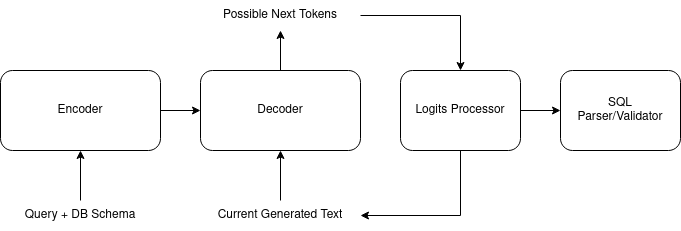
\includegraphics[width=\textwidth]{t5-transformer.drawio.png}
\caption{\label{fig:model} Model Overview}
\end{figure*}

The goal of this project was to assess the production viability of generating SQL from a natual language query for a common REST server. The model itself needed to be proven to be effective in a general sense and against a real database for a real use case. The integration of the model into the application also needed to account for the possibility of many concurrent users. It is also hoped that the model can be used in a general-purpose manner so that it can be quickly adapted to whatever use case it might be beneficial for.

The \texttt{T5} model \citep{raffel2020exploring} is short for Text-to-Text Transfer Transformer and is one of the beginning auto-regressive Transformer models for text generation. It was created by Google in 2020 following \texttt{GPT-2} in 2019 \citep{radfordgpt2} and served as their solution for translation and summarization tasks in the wake of the shift to transformers from Recurrent Neural Networks. The \texttt{T5} has since been replaced at Google by \texttt{FLAN-T5} \citep{chung2022scaling} and \texttt{PaLM} \citep{chowdhery2022palm}, but still remains as one of the state of the art models used for Text-to-SQL generation.

Despite there being models that are technically better than the \texttt{T5} model, we still used it for our assessment because it has been proven to work for our needs. The major difference in our task versus the others in this space is that our demo application requires the generated SQL to target a predetermined table and produce a predetermined set of columns. Another reason the \texttt{T5} model is a good choice is that this requirement is easily able to be solved by any auto-regressive Transformer as long as it is paired with a constrained decoder.

% Evaluation (explain how you answered your question and how your evaluation substantiates that claim, also discuss the limitations of your work--what can you reasonably expect it to do and not to do)
\section{Evaluation} \label{sec:eval}


\subsection{Task \& Procedure}

\subsubsection{Model}

We started our efforts with a \texttt{T5} model that was already fine-tuned by the Picard project \citep{scholak2021picard}. This model was used because it is one of the state of the art models in this area of study and is easy to build off of due to its compatibility with Huggingface \citep{wolf2020huggingfaces}. We also benefitted from this model's database schema agnosticity because it expects the target database schema as an input and that meant that further fine-tuning to support a particular database is unnecessary. This is the main reason that no further fine-tuning was done.

We augmented this model by pairing it with a custom Huggingface Logits Processor that utilizes a \texttt{PyParsing} PostgreSQL SQL grammar \citep{githubPyparsing} to parse the generated SQL and ensure the chosen tokens contribute to a valid SQL output. This was done to implement a constrained decoder for our model and is useful because it helps ensure that the overall generated SQL is valid. We could have used Picard's Logits Processor, but chose not to because their solution utilized Haskell and thus would have been difficult to modify. Figure~\ref{fig:model} illustrates how the Transformer, Logits Processor and SQL parser work in tandem.

A constrained decoder approach is useful for text generation with Transformers that are meant for a specialized task like code generation. A model can be trained to do a lot of things, but it's debatable how perfect of a job it can do in all situations. A constrained decoder fills in the gaps by steering the text generation in the right direction. It can even be argued that a constrained decoder allows for a smaller model, with less parameters. Picard's constrained decoder for instance knows more details about the target database schema than what is provided in the inputs to the encoder and can thus make sure the proper operators and literals are used based on the type of table columns that they are being used alongside.

In addition to a custom Logits Processor, we also added a forced prefix to the generated SQL output by utilizing Huggingface's support for a restricted vocabulary. This was done to ensure that the generated SQL targeted the expected table and outputted the expected columns. Our demo application relied on this behavior due to the assumption that the generated SQL would always target a predetermined table and would return all of the columns related to that table. Our constrained decoder strategy likely wouldn't have been possible without the auto-regressive nature of our model and wouldn't have met our requirements for generating valid SQL that retrieves predetermined information.

For the general evaluation of this model we utilized the \texttt{Spider Text-to-SQL} dataset \citep{yu2019spider} to verify that the model by itself is capable of generating reasonable SQL results. This was done in a unit test environment.

We also relied on a human evaluation for our demo application as a whole. Refer to Figure~\ref{fig:architecture} for an idea of the overall architecture. This was necessary to evaluate how well our Text-to-SQL strategy worked against a real database for a real use case. Part of the evaluation was determining what was necessary to utilize the generated SQL for real database queries, while the other part was validating that the generated SQL made sense based on the natual language queries that we used for our movie database.

\begin{figure}
\centering
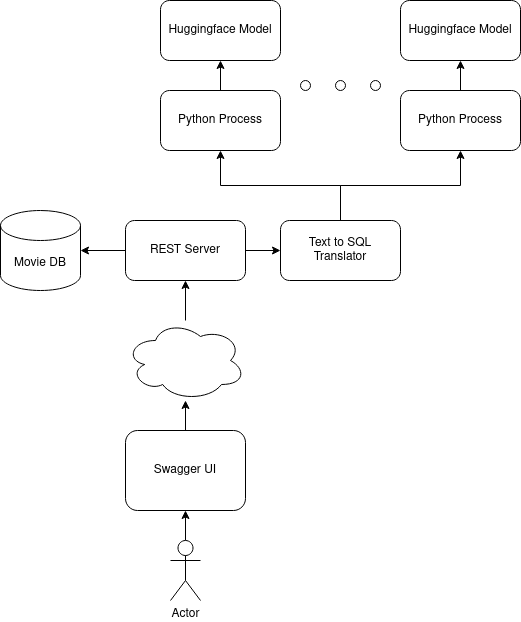
\includegraphics[width=0.5\textwidth]{demo-architecture.drawio.png}
\caption{\label{fig:architecture} Demo Architecture}
\end{figure}

\subsubsection{Framework}

The model was a core effort for this project, but the framework around that model is equally important. In order for the model to be useful in a production environment it needs to support multiple users to some degree. This ultimately needed to be a focus of the project to assess production viability.

The approaches explored for scalability included spawning Python processes with their own model based on the load of the application and utilizing batching for the queries. Figure~\ref{fig:architecture} illustrates the overall architecture for the demo application. The \texttt{Text to SQL Translator} piece was written to be a separate library that can be stood up on multiple computers if necessary and its main feature is that it spawns worker Python processes with our model based on the translation load. This was accomplished using Deep Java Library's model serving utility \citep{djlserving}.

DJL does a lot of things, but its serving utility claims to automatically support scaling up/down workers based on the load and dynamically batching requests. Although, these features weren't fully explored and evaluated in this project, we still have incorporated its usage into the overall project with the assumption that its features work as expected. More exploration is required for how this library can be configured to fully accomplish a production environment's scaling needs while taking to account excessive RAM usage of the models and ensuring batch sizes aren't too large.

\subsubsection{Metrics}

The various evaluation efforts used in this project required different metrics tailor made for each of the strategies. The main evaluation utilized the Spider dataset to test the quality of the generated SQL and the results were measured using a content overlap algorithm. We knew what sequence of tokens were expected to be in the resulting query and also which tokens were actually present in the generated SQL. Therefore the resulting content overlap was measured as an overall percentage of the expected tokens that matched the actual results. A side effect of this strategy is that the expected queries with a high amount of tokens contributed more to the resulting percentage than expected queries with less tokens.

\subsubsection{Results}

The work explored in this project could easily be developed into a general-purpose library that has potential for being commonly used by any application that requires information to be retrieved from a database based on a user's needs. In the same way ORMs are designed to make database storage easier, this work makes the job of translating a user's request into the information that they wish to see easier. However, much like with ORMs this solution isn't going to replace the SQL that an expert is capable of writing for use cases that require efficient/performant queries and complete accuracy of the results. This approach will satisfy most of a user's needs, but will likely never be the right tool for every use case in the same way that the UDP protocol isn't the right tool for all communication.

The final percentage that we achieved for the Spider dataset evaluation was about \texttt{61.2\%} and that again represents the percentage of the total expected tokens matching what was in the generated SQL. The Picard project was able to achieve a higher percentage than ours at \texttt{74.8\%}, but also had a much better constrained decoder implementation that took into account the actual data types of the columns in the target database schema. Their incremental parser was also probably better in general as well.

The human evaluation of the overall demo application didn't necessarily have results that can be measured, but we have observed some interesting details and obstacles. Unlike the Spider evaluation, the demo application requires that the generated SQL has a predetermined set of column outputs and targets a particular table. In hindsight, forcing a prefix worked but also artificially gave the decoder some unintended cues towards what the rest of the SQL should include. With the anticipation that the generated SQL might generate a \texttt{JOIN} clause, the forced prefix included an alias to the main table that was to be queried. This resulted in almost all of the generated SQL containing a \texttt{JOIN} clause regardless of its actual necessity and usage in the rest of the query. It's possible that the training data would need to be adapted to correct this minor issue.

In the development of the model, we have also observed that the model and SQL parser can sometimes get into states where they appear to ``argue'' with each other over what parts of the SQL is and isn't valid. This mostly occurs when incremental parsing is enabled instead of only parsing the generated SQL when an end token is encountered. The only explanation we have is that the parser isn't failing fast enough during the generation due to how lenient it was written in order to account for partial word token, which when observed by themselves may be seen as invalid. If the parser confirms that a partial word token is valid in one pass and then invalid when the next token completes the word, then it's believable that the generation process might get into a state of confusion. In these situations the generated SQL usually grows to be very large and we timeout before the end of the sequence is reached.

% Implications (who would use your work? who does it affect? would it affect anyone in a negative way?)


%\begin{figure}
%\centering
%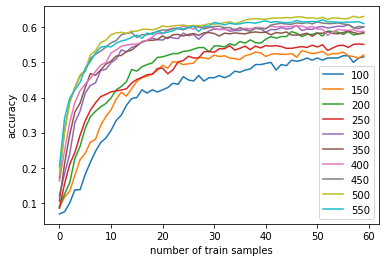
\includegraphics[width=0.5\textwidth]{figures/bert_funcs2emotions.png}
%\caption{\label{fig:results} Results for experiment 1: }
%\end{figure}

%Figure~\ref{fig:results} shows the results.

%Talk objectively about what you observe.


% Conclusion (bring everything together and write a concise take-home message)
\section{Conclusion}

%Explain more about your results and what they suggest.

\subsection{Implications}

%What do your results mean?

\subsection{Limitations}

%One limitation is ... the training data and test data could have some overlap ...


\subsection{Future Work}


% Attached is an example submission that is worth emulating (you are not required to use multiple columns)


\cite{scholak2021picard}

\cite{wolf2020huggingfaces}

\cite{yu2019spider}

\cite{misc_movie_132}


% Entries for the entire Anthology, followed by custom entries
\bibliography{custom}

% \appendix

% \section{Example Appendix}
% \label{sec:appendix}

% This is a section in the appendix.

\end{document}
